\documentclass[a4paper,12pt,bibliography=totoc]{scrreprt}% ohne Option toc=flat
\usepackage{tocstyle}
\usetocstyle{allwithdot}
\usepackage{lmodern}
\usepackage{natbib}
\usepackage{graphicx} 
\usepackage{subfigure} 
\usepackage[hyphens]{url}
\usepackage[utf8]{inputenc}% Kodierung
\usepackage[ngerman]{babel}% Sprache
\usepackage{filecontents}
\begin{filecontents}{books.bib}

@MISC{winrichtlinien,
	author = "{Microsoft Corporation}",
	year = "2014",
	title = "Windows App Development: Guidelines for targeting",
	howpublished = "\url{http://msdn.microsoft.com/en-us/library/windows/apps/hh465326.aspx}",
	note = "Abrufdatum: 06.08.2014"
}

@MISC{applerichtlinien,
	author = "{Apple Inc.}",
	year = "2014",
	title = "iOS Human Interface Guidelines: Layout",
	howpublished = "\url{https://developer.apple.com/library/ios/documentation/UserExperience/Conceptual/MobileHIG/LayoutandAppearance.html}",
	note = "Abrufdatum: 09.08.2014"
}

@MISC{androidrichtlinien,
	author = "{Open Handset Alliance™}",
	year = "2014",
	title = "Android Developers: Metrics and Grids",
	howpublished = "\url{http://developer.android.com/design/style/metrics-grids.html}",
	note = "Abrufdatum: 09.08.2014"
}

@MISC{sonyverge,
	author = "Dante D'Orazio",
	year = "2012",
	title = "Sony Xperia Sola's 'floating touch' screen technology explained",
	howpublished = "\url{http://www.theverge.com/2012/3/14/2871193/sony-xperia-sola-floating-touch-hover-event-screen-technology}",
	note = "Abrufdatum: 07.08.2014"
}

@ARTICLE{monkeys,
  author = "Dandekar, K., Raju, B.I. and Srinivasan, M.A.",
  title = "3-D finite-element models of human and monkey fingertips to investigate the mechanics of tactile sense",
  pages = "682-691",
  journal = "Journal of biomechanical Engineering",
  volume = "125"
}

@INCOLLECTION{jin,
  author = "Zhao Xia Jin, Tom Plocher, Liana Kiff",
  title = "Touch screen user interfaces for older adults: button size and spacing",
  booktitle = "Proceedings of the 4th international conference on Universal access in human computer interaction: coping with diversity (UAHCI'07)",
  publisher = "Springer Verlag",
  year = "2007",
  editor = "Constantine Stephanidis",
  pages = "933-941",
  address = "Berlin, Heidelberg"
}

@ARTICLE{touchmouse,
  author = "Charlotte Travis and Pietro Murano",
  title = "A comparative study of the usability of touch-based and mouse-based interaction",
  journal = "Int. J. Pervasive Computing and Communications",
  volume = "10",
  number = "1",
  year = "2014",
  pages = "115-134"
}

\end{filecontents}

%############## BEISPIELE
%INTERNETSEITE###############
% @inproceedings{inhaus,
%    author={Klaus Scherer},
%    title={Das Potenzial intelligenter Haustechnik
% für ehome-care},
%    publisher={Präsentation auf der ZTG-Tagung am 09.05.2006, Krefeld},
%    year={2006}
%}
%
%INTERNETSEITE###############
%@book{rfid,
%  title={RFID-Handbuch: Grundlagen und praktische Anwendungen von Transpondern,  % kontaktlosen Chipkarten und NFC},
%  author={Finkenzeller, K.},
%  isbn={9783446412002},
%  year={2008},
%  publisher={Hanser, Carl}
%}
%
%INTERNETSEITE###############
%@incollection{lev1,
%  author={Lev Manovich},
%  title={Die Poetik des erweiterten Raumes},
%  pages={337-349},
%  booktitle={Topos Raum: Die Aktualit{\"a}t Des Raumes in Den K{\"u}nsten Der %Gegenwart},
%  editor={Lammert, A. and {Akademie der K{\"u}nste Berlin}},
%  isbn={9783938821077},
%  lccn={2006483669},
%  year={2005},
%  publisher={Verlag f{\"u}r Moderne Kunst},
%  address={Nürnberg}
%}
%
%INTERNETSEITE###############
%@misc{linden,
%year = 2012,
%  key = {linden},
%  title = "ABOUT LINDEN LAB",
%  howpublished="\url{http://lindenlab.com/about}",
%note="Abrufdatum: 10.09.2012"
%}
%
%INTERNETSEITE MIT AUTHOR##############
%@misc{stereo,
%year = 1997,
%  author ="{van Ackern}, N. and Lindenberg, Markus",
%   title = "Räumliches Hören",
%  howpublished="\url{http://irtel.uni-mannheim.de/lehre/seminararbeiten/w96/Hoeren1/Hoeren1.html}",
%note="Abrufdatum: 27.03.2012"
% }

\usepackage[T1]{fontenc}
%PHONE LETTER SYMBOLS
\usepackage{pifont}
%Das Paket wird fuer die anderthalb-zeiligen Zeilenabstand benštigt
\usepackage{setspace}
%Abstand eines neuen Absatzes
\setlength{\parskip}{1em}
\setlength{\parindent}{0em}
%Definition der Raender
\usepackage[paper=a4paper,left=30mm,right=30mm,top=30mm,bottom=30mm]{geometry}
%Abstand der Fussnoten
\deffootnote{1em}{1em}{\textsuperscript{\thefootnotemark\ }}
%Regeln, bis zu welcher Tiefe (section,subsection,subsubsection) Überschriften angezeigt werden sollen (Anzeige der berschriften im Verzeichnis / Anzeige der Nummerierung)
\setcounter{tocdepth}{3}
\setcounter{secnumdepth}{3}
%-------------------
%Ende des Kopfbereiches
%-------------------

%-------------------
%Hier beginnt der Text deiner Hausarbeit
%-------------------
\begin{document}
%Beginn der Titelseite
\begin{titlepage}
\begin{center}
\null
\vfill
\begin{Large}
\textsf{\textbf{Untersuchung der Usability von Hover-Erkennung auf Smartphones.}}
\end{Large}\linebreak \linebreak 
\begin{large}
\textsf{Auswirkungen der Hover-Erkennung auf die Präzision und Geschwindigkeit bei Interaktionen auf mobilen Endgeräten.}
%Empirische Untersuchung mittels eines Prototypen zur Ermittlung von Auswirkungen der Hover-Erkennung auf Präzision und Geschwindigkeit bei Interaktionen auf mobilen Endgeräten.
\end{large}
\begin{small}
\vfill{Jan-Hendrik Wolf \\ Matrikelnummer: 2616233 \\ Mainstraße 36 \\  28199 Bremen \\\ding{38} 0151 15530761\\\ding{41} mail@jan-wolf.de \\\vspace{3cm} Universität Bremen\\ Digitale Medien B. Sc. \\ Sommersemester 2014}
\null
\end{small}
\end{center}
\end{titlepage}
%Ende der Titelseite

%Inhaltsverzeichnis (aktualisiert sich erst nach dem zweiten Setzen)
\tableofcontents
\thispagestyle{empty}
%Beginn einer neuen Seite
\clearpage
%Anderthalbzeiliger Zeilenabstand ab hier
\onehalfspacing
\pagestyle{plain}

%START-----------------------------------------------------------------------------------
\chapter{Zusammenfassung}
Zusammenfassung der GESAMTEN Arbeit.

\chapter{Einleitung}
Die Interaktion auf mobilen Endgeräten rückt durch deren stetigen Verbreitung in den letzten Jahren verstärkt in den Fokus. Neben den etablierten Interaktionsformen für Maus und Tastatur an Desktop-Computern steigt der Einfluss alternativer und für den mobilen Einsatz geeigneter Varianten zunehmend an.
Aufgrund der bisherigen, technischen Beschränkungen auf berührungsempfindlichen Bildschirmen wurden die Interaktionen auf Bedienelemente neben peripheren Sensoren, wie z.B. Neigungs- oder Lichtsensoren, bisher jedoch ausschließlich durch direkte Bildschirmberührungen realisiert.

Trotz der sinnvollen Eigenschaften wurde wohl aus den genannten Gründen auch das sogenannte "`Hovering"' nicht in das Repertoire der Interaktionsformen mobiler Endgeräte übernommen.
Als "`Hovering"' bezeichnet man das Schweben mittels der Maus an einem Laptop oder Desktop-Computer über einem Objekt auf der Benutzungsoberfläche, welches anschließend und je nach Eigenschaft sein Aussehen verändert, sodass der Nutzer das Objekt beispielsweise als Schaltfläche identifizieren kann.\\
Durch diese fehlende Interaktionsform erweist sich das Selektieren und Auswählen von kleinen Bedienelementen als schwieriger, da der Finger der Nutzer das Bedienelement zu einem großen Teil überdecken kann. Um dem "`Fat-Finger-Problem"' \cite{monkeys} entgegenzuwirken, ist die Mindestgröße der Bedienelemente auf berührungsempfindlichen Bildschirmen im Vergleich zu Bedienelementen für Mausinteraktionen vergrößert worden \cite{jin}.

Nachdem Sony im Mai 2012 erstmals ein Smartphone mit integrierter Annäherungserkennung für den gesamten Markt veröffentlichte, war es nun technisch möglich diese neue Interaktionsform auf einer Benutzungsoberfläche anzuwenden \cite{sonyverge}. Die Integration der Annäherungserkennung erfolgt dabei jedoch in einem mäßigen Tempo und ist zum heutigen Stand nur in einem kleinen Teil der Geräte erfolgt.

In der bevorstehende Bachelorarbeit soll untersucht werden, ob visuelle Hover-""Effekte auf berührungsempfindlichen Endgeräten mit integrierter Annährungserkennung die Usability von Bedienelementen im Bezug auf Geschwindigkeit und Präzision verbessern kann und auf diese Weise eine beschleunigte Integration dieser Technologie gerechtfertigt werden kann.

\section{Gegenwärtiger Stand der Technik mobiler Endgeräte}
Zum jetzigen Zeitpunkt ist die Anzahl der Geräte mit integrierter Annäherungsfunktion stark begrenzt. Zudem nutzen die Benutzungsoberflächen auf heutigen Smartphones mit Annährungserkennung die Möglichkeiten der Technologie nur in vereinzelten Fällen aus. Im Folgenden soll ein kurzer Überblick auf die gegenwärtige Hardware und Software gegeben werden, die diese Annäherungserkennung unterstützt.

\subsection{Hardware}
Nachdem Sony im Jahr 2012 mit dem Xperia™ sola das erste Mal ein Smartphone mit Annäherungserkennung unter dem Namen Floating Touch™  veröffentlichte, bot auch der Smartphone-Hersteller Samsung zu Beginn des Jahres 2013 ein Gerät mit ähnlicher Technologie namens AirView™ auf den Markt. Bei beiden Geräten handelte es sich jedoch nicht um Einsteigergeräte, sondern waren im mittleren bis hohen Preissegment vertreten. Im Gegensatz zu Sony, integrierte Samsung im Jahr 2014 die Annäherungserkennung auch in das Nachfolgermodell, dem Samsung Galaxy S5.

\subsection{Software}
In den bisherigen mobilen Endgeräten mit integrierter Annäherungserkennung wurden unterschiedliche Ansätze zur Nutzung dieser Technologie in Benutzungsoberflächen realisiert.\\
Sony nutzte die Technologie, um Hintergrundbilder auf dem Hauptbildschirm zu bewegen und der Nutzer somit direkten Einfluss auf das Verhalten hat. Zusätzlich wurde der interne Browser des Smartphones modifiziert, sodass die Annäherungserkennung auf Webseiten genutzt werden konnte. Somit konnten mit den auf Webseiten häufig verwendeten und auf Annäherung sensiblen Bedienelementen erneut im vollen Umfang interagiert werden.

Der Hersteller Samsung bietet in dessen Smartphones ebenfalls mehrere Anwendungen an, die auf Annäherung reagieren. Sie lassen sich in zwei Arten unterteilen: In der Ersteren werden Informationen auf kleinem Raum durch Annäherung vergrößert bzw. neu angeordnet, sodass sich die Übersicht für den Nutzer verbessert. Als Beispiel dient hier die Gallerieanwendung, siehe Abbildung \ref{samsungeinleitung1}. In der Gallerie werden Bilder bei Annäherung vergrößert, sodass der Nutzer eine Vorschau erhält.

\begin{figure}
\subfigure[Normalzustand der Galerie]{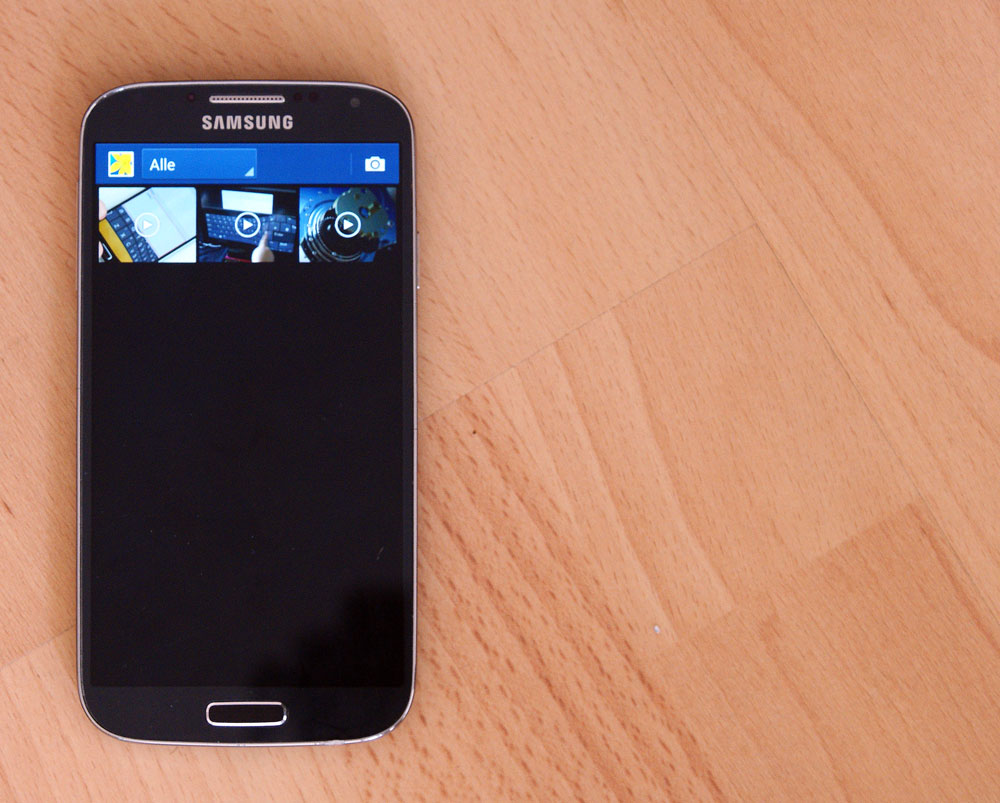
\includegraphics[width=0.49\textwidth]{img/nohover.jpg}}
\hfill
\subfigure[Bildvergrößerung bei Annäherung]{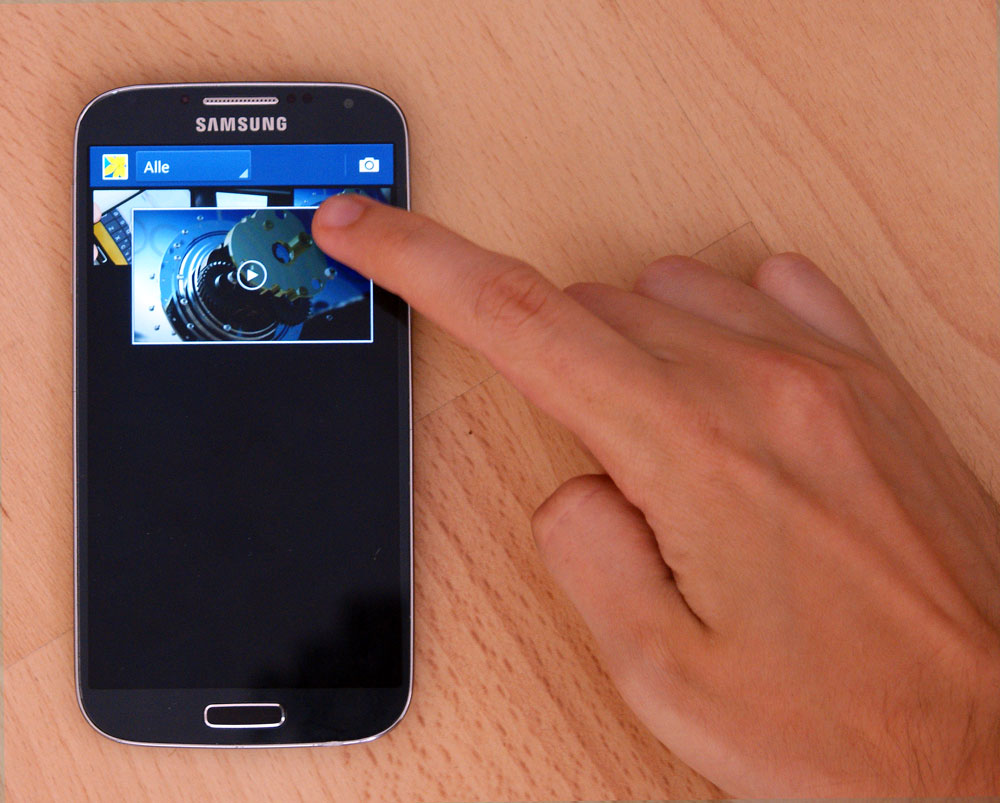
\includegraphics[width=0.49\textwidth]{img/hover.jpg}}
\caption{Objektvergrößerungen bei Annäherung mit aktiviertem AirView™ auf einem Samsung Galaxy S4.}
\label{samsungeinleitung1}
\end{figure}

Die zweite Art der Anwendungen zeigen bei Annäherung nicht Vergrößerungen oder detaillierteren Ausführungen, sondern zuvor nicht sichtbare Informationen an, siehe Abbildung \ref{samsungeinleitung2}. Somit können weitere Zusatzinformationen eingeblendet werden. Als Beispiel dient die Wählanwendung, in der bei Annäherung auf eine aktive Kurzwahltaste der darauf jeweils gespeicherte Kurzwahlkontakt angezeigt wird.

\begin{figure}
\subfigure[Normalzustand des Wahlbildschirms]{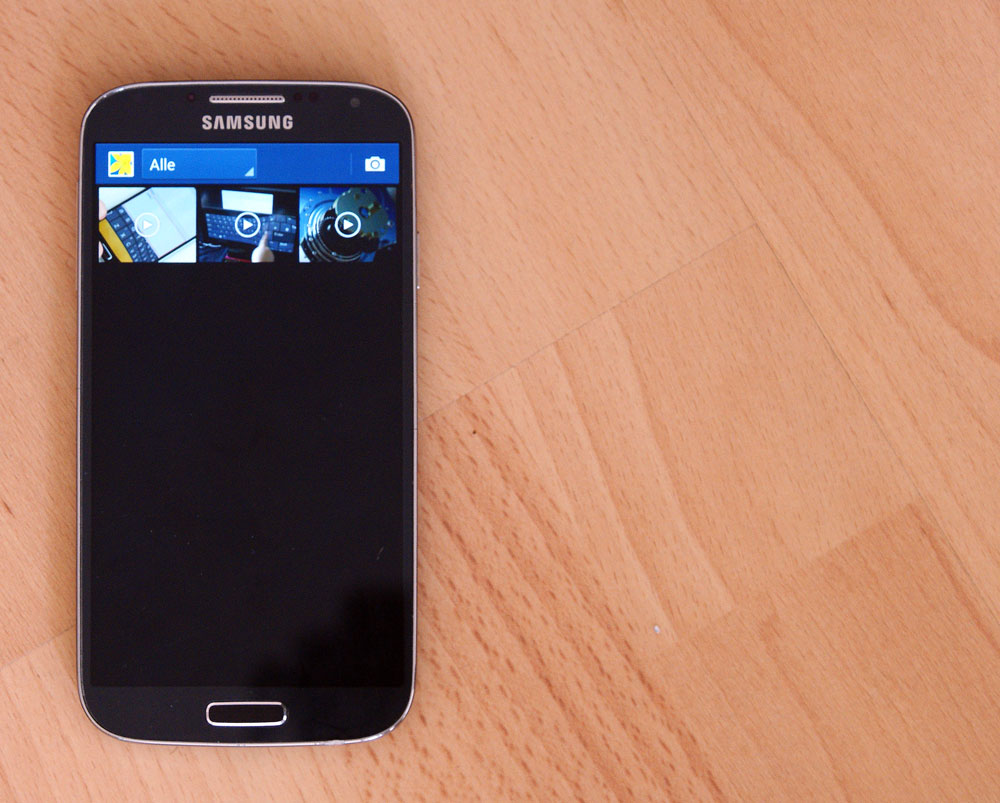
\includegraphics[width=0.49\textwidth]{img/nohover.jpg}}
\hfill
\subfigure[Kurzwahlinformationen bei Annäherung]{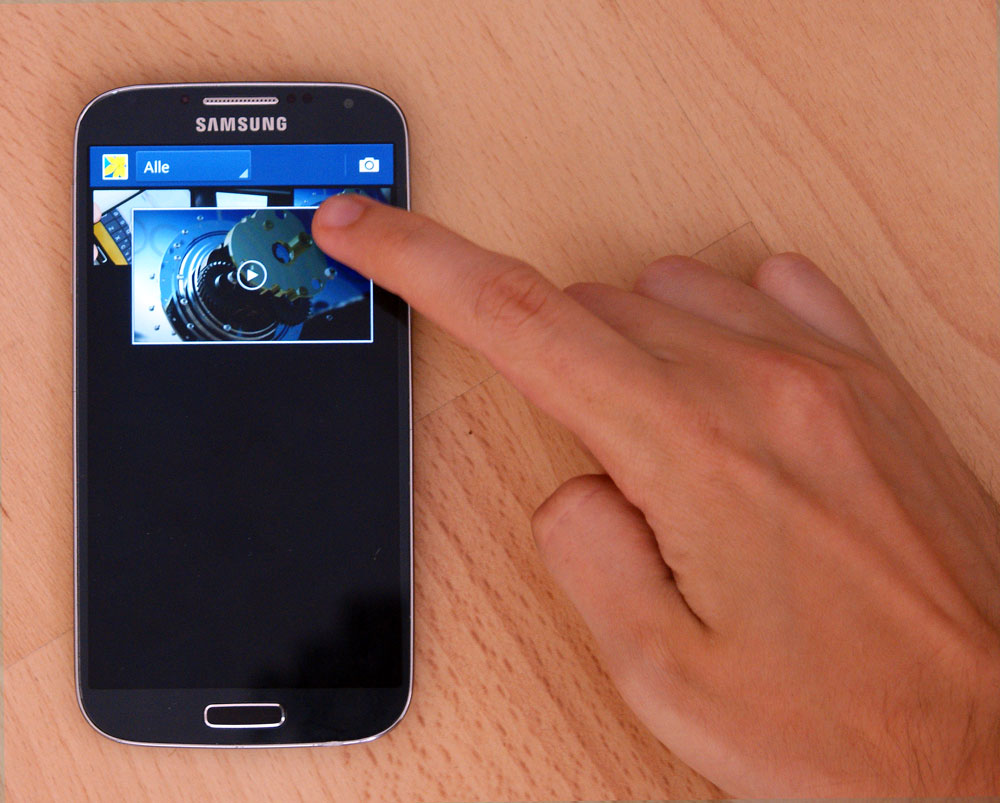
\includegraphics[width=0.49\textwidth]{img/hover.jpg}}
\caption{Einblenden zusätzlicher Informationen bei Annäherung auf einem Samsung Galaxy S4 mit aktiviertem AirView™.}
\label{samsungeinleitung2}
\end{figure}

\section{Bisherige Leitfäden für Bedienelemente}
Aufgrund der geringeren Abmessungen mobiler Endgeräte ist die Gestaltung der Bedienelemente ein entscheidendes Kriterium für die reibungslose Interaktion zwischen Mensch und Maschine. Alle Hersteller der populären mobilen Betriebssysteme bieten umfangreiche Leitfäden zur Gestaltung von Bedienelemente für Anwendungsentwickler an.
In diesen Leitfäden werden u.A. Mindestangaben zu Größen und Abständen kommuniziert. Dabei sind die Mindestgrößen für Bedienelementen in diesen Leitfäden im Vergleich zu Desktop-Computer sehr viel größer. Studien haben ergeben, dass Nutzer mit Mausinteraktionen gegenüber Berührungsinteraktionen präziser und schneller arbeiten. Darüber hinaus wird die Interaktion mit der Maus bei Aufgaben, die genaue Selektionen benötigen, bevorzugt \citep{touchmouse}. 
Die Tabelle \ref{leitfadenalle} zeigt zur Veranschaulichung die in den Leitfäden empfohlenen Mindestgrößen der unterschiedlichen Hersteller.

\begin{table}
\centering
\renewcommand{\arraystretch}{1.5}
\setlength{\tabcolsep}{15pt}
\begin{tabular}{ l c c }
Plattform & Minimale Größe & Empfohlene Größe\\\hline
Android \cite{androidrichtlinien} & 7mm & 9mm\\
Apple \cite{applerichtlinien} & 7mm & 7mm\\
Windows \cite{winrichtlinien} & 7mm & 9mm\\
\end{tabular}
\caption{Mindestgrößen von Bedienelementen.}
\label{leitfadenalle}
\end{table}


\chapter{Methodik}


\section{Testpersonen}


\section{Apparat}


\section{Kalibrierung}
Aufgrund der technischen Eigenschaften, die bei der Ermittlung des Fingers während der Schwebeposition bestehen, ist eine mögliche Ungenauigkeit im Vergleich zur tatsächlichen Fingerposition denkbar. Gleichzeitig kann je nach Anstellwinkel des Fingers der dichteste Punkt zum Bildschirm variieren und möglicherweise zusätzliche Ungenauigkeiten erzeugen. Beim internen Testen des Prototypen zeigten sich teilweise deutliche Unterschiede zwischen den Schwebe- und Klickpositionen. Resultierend daraus wurden die kleinen Quadrate im zweiten Testteil nicht mehr hervorgehoben, bevor diese schließlich berührt werden würden.

Um die Verschiebungen zwischen der Schwebe- und Klickposition des Fingers nachzuvollziehen, wurde dem Testprototypen eine zusätzliche Ebene innerhalb der Benutzungsoberfläche hinzugefügt, die die letzte Klick- und Schwebeposition anhand von Kreuzen sichtbar machte. Bei internen Versuchen bestimmte Bereiche des Testprototypen anzuklicken, wurde deutlich, dass die beiden Kreuze nicht aufeinander lagen, sondern sich in vielen Fällen in ihrer Position unterschieden.

Um mögliche Zusammenhänge der Verschiebungen zwischen der Schwebe- und Klickposition des Fingers nachzuweisen, wurde eine Testanwendung implementiert, die die letzte Schwebe- und Klickposition aufzeichnete. Dabei sollten Nutzer in der Arbeitsgruppe, in der ich die Bachelorarbeit verfasst, eine Abfolge von verschiedenen Punkte auf dem Bildschirm berühren. Die jeweiligen Schwebe- und Klickpositionen waren für die Testperson waren zu diesem Zeitpunkt nicht sichtbar und wurden erst nach dem eigentlichen Test visualisiert. Anschließend wurden die Werte mittels einen eigens geschriebenen Hilfsprogramm geplottet und ausgewertet.

\begin{figure}
\subfigure[Interaktion mit dem Finger]{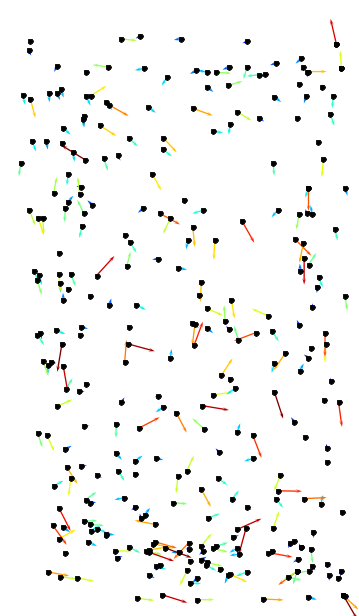
\includegraphics[width=0.45\textwidth]{img/kalibrierung_finger.png}}
\hfill
\subfigure[Interaktion mit dem Daumen]{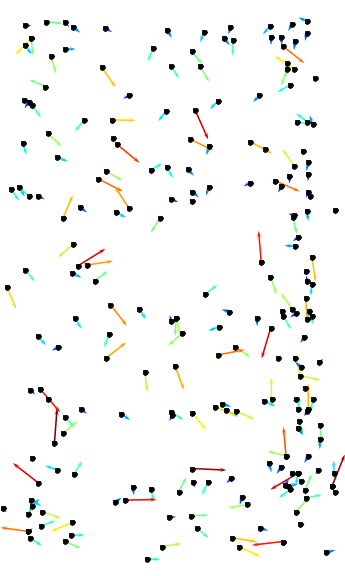
\includegraphics[width=0.45\textwidth]{img/kalibrierung_daumen.png}}
\caption{Visualisierung der relativen Verschiebungen zwischen der Klick- und Schwebeposition. Die Pfeile inkl. Farbtemperatur deuten die Distanz der Verschiebung an.}
\label{klickschwebepositionen}
\end{figure}

Die Abbildung \ref{klickschwebepositionen} zeigt die relativen Verschiebungen zwischen der Klick- und Schwebeposition an und verdeutlicht gleichzeitig die teilweise sehr starken Schwankungen beider Werte.
Obwohl an mehreren stellen Tendenzen zur Verschiebungsrichtung erkennbar sind, besitzen die Werte dennoch eine große Varianz. Die Möglichkeit die Schwebepositionen auf die Klickpositionen zu verschieben (und andersherum) wären theoretisch möglich, z.B. durch lineare oder polygonale Regression. Da die Ermittlung dieser Variablen den Umfang dieser Bachelorarbeit jedoch übersteigen würde, wird eine Kalibrierung im Rahmen dieses Tests nicht verfolgt.

\section{Prozedur}


\section{Design}


\chapter{Ergebnisse}


\section{Test 1: Listenauswahl}


\section{Test 2: Präzisionstest}


\section{Vergleich zu den bisherigen Leitfäden}


\chapter{Fazit}


\section{Ausblick}
Multi-Hover-Touch
Lorem Ipsum hier kommt die Fazipsum.

\chapter{Danksagung}
Kurze Danksagung für Bachelorarbeit und Studium.

%ENDE-----------------------------------------------------------------------------------
%Beginn einer neuen Seite
\clearpage
\bibliographystyle{plain}
\bibliography{books}
\newpage
\addcontentsline{toc}{chapter}{Erklärung}
\chapter*{Erklärung}
Ich versichere hiermit, dass ich die vorliegende Facharbeit selbständig verfasst und keine anderen als die angegebenen Quellen und Hilfsmittel benutzt habe. Die Arbeit wurde keiner anderen Prüfungsbehörde vorgelegt und auch nicht veröffentlicht.
\begin{center}
\begin{tabular}{lp{2em}l} 
 \hspace{5cm}   && \hspace{4cm} \\\cline{1-1}\cline{3-3} 
 Bremen, \today    && Jan-Hendrik Wolf 
\end{tabular} 
\end{center}
\end{document}
%-------------------
%Hier endet der Text der Bachelorarbeit.
%-------------------